\documentclass[conference]{IEEEtran}
\IEEEoverridecommandlockouts
\usepackage{mathptmx} % Times for text and math: one font family throughout
\usepackage{cite}
\usepackage{amsmath,amssymb,amsfonts}
\usepackage{algorithm}
\usepackage{algpseudocode}
\makeatletter
\let\oldfsruled\fs@ruled
\renewcommand\fs@ruled{\oldfsruled\def\@fs@cfont{\normalfont}}
\makeatother
\restylefloat{algorithm}
\usepackage{graphicx}
\usepackage{booktabs}
\usepackage{multirow}
\usepackage{xcolor}
\usepackage{tikz}
\usetikzlibrary{positioning,arrows.meta,fit}
\usepackage[hidelinks]{hyperref}
\usepackage{balance}
\usepackage{amsthm}
\newtheoremstyle{plainhead}{3pt}{3pt}{\itshape}{}{\normalfont}{.}{.5em}{}
\theoremstyle{plainhead}
\newtheorem{proposition}{Proposition}
\algrenewcommand\algorithmicrequire{Require:}
\algrenewcommand\algorithmicfor{for}
\algrenewcommand\algorithmicdo{do}
\algrenewcommand\algorithmicend{end}
\algrenewcommand\algorithmicreturn{return}
\algrenewcommand\algorithmicwhile{while}
\algrenewcommand\algorithmicif{if}
\algrenewcommand\algorithmicthen{then}

\newcommand{\iws}{\textsc{IWS}}
\newcommand{\pp}{\,pp}

\begin{document}

\title{When Does a Machine Learning Model Fail?\\
Linking Feature-Space Changes to Prediction Degradation}

% ---- Replace with your details (remove for double-blind review) ----
\author{\IEEEauthorblockN{First Author}
\IEEEauthorblockA{\textit{Department} \\
\textit{Institution}\\
City, Country \\
email@domain}
\and
\IEEEauthorblockN{Second Author}
\IEEEauthorblockA{\textit{Department} \\
\textit{Institution}\\
City, Country \\
email@domain}}

\maketitle

\begin{abstract}
Deployed models are routinely monitored with drift detectors that raise an alarm whenever the input distribution changes, yet a change in $P(X)$ need not change the error of the model. We ask which measurable feature-space changes actually predict prediction degradation, and why the rest do not. We assemble a testbed of 173 natural source$\to$target shifts drawn from seven public tabular datasets (demographic, geographic, temporal and carrier splits), train three model classes with three seeds each (1{,}557 evaluations), and compare thirteen label-free signals against the true accuracy drop. We also propose \emph{Importance-Weighted Shift} (\iws{}), which weights each feature's drift by the model's own reliance on that feature, and a reweighting decomposition that separates the covariate part of a drop from the conditional part. Three findings stand out. First, drift is nearly universal but weakly informative: a domain classifier separates source from target with AUC $\ge 0.95$ in 68\% of pairs, while 25\% of drifted evaluations show no harm and 48\% of low-drift evaluations still fail. Second, \iws{} gives the best harm detection among single signals (AUROC 0.70, AUPRC 0.86) and the highest rank correlation with the drop ($\rho=0.42$), whereas confidence-based estimators that work well on images correlate weakly on tabular shifts ($\rho \approx 0.07$). Third, in 76\% of harmful evaluations the conditional part $P(Y|X)$ dominates the covariate part, and controlled experiments confirm that such concept shift is invisible to every label-free signal. We release code and results to support reproducible monitoring research.
\end{abstract}

\par\vspace{4pt}\noindent{\normalfont\small\textit{Index Terms}---
distribution shift, concept drift, model monitoring, performance estimation, tabular data, feature importance}\par

% =====================================================================
\section{Introduction}
% =====================================================================
A model that was accurate at validation time can quietly lose accuracy after deployment because the data it receives no longer resembles the data it was trained on~\cite{quinonero2009dataset,moreno2012unifying}. Labels that would reveal the loss usually arrive late or never, so practitioners rely on \emph{drift detectors}: univariate tests such as Kolmogorov--Smirnov (KS) or the Population Stability Index (PSI), kernel two-sample tests~\cite{gretton2012kernel}, or classifier two-sample tests~\cite{lopezpaz2017c2st,rabanser2019failing}. These tools answer the question ``has $P(X)$ changed?''. The question an operator actually needs answered is different: ``will my model now make more mistakes?''.

The two questions come apart for two reasons. A change confined to features the model ignores is harmless, yet it triggers every detector. Conversely, a change in the relation between features and label, $P(Y|X)$, can destroy accuracy while leaving $P(X)$ untouched, so no detector fires. Recent work on tabular benchmarks found that such conditional shifts are common in practice~\cite{liu2023need}, and that the accuracy gap tracks label-distribution shift~\cite{gardner2023tableshift}. What is missing is a direct, large-scale measurement of how well each label-free signal predicts the actual drop, and of \emph{why} it fails when it does.

This paper provides that measurement and makes four contributions:
\begin{enumerate}
  \item \textit{A shift--degradation testbed.} 173 natural source$\to$target pairs from seven public tabular datasets, three model classes, three seeds, 1{,}557 evaluations, each with its true accuracy drop and 13 label-free signals.
  \item \textit{Importance-Weighted Shift (\iws{}).} A simple model-aware statistic that weights per-feature drift by permutation importance. It is the best single predictor of harm in our testbed and costs one importance computation per deployed model.
  \item \textit{A covariate/conditional decomposition} of each drop by density-ratio reweighting, validated on synthetic shifts with known ground truth, showing that conditional shift dominates natural tabular failures.
  \item \textit{A failure taxonomy} (stable, benign drift, harmful covariate shift, conditional failure) with practical guidance on when a drift alarm should trigger retraining.
\end{enumerate}

% =====================================================================
\section{Related Work}
% =====================================================================
\textit{Shift detection.} Classical concept-drift research monitors streams for changes~\cite{gama2004ddm,gama2014survey,lu2019learning,webb2016characterizing}. For batch shift, Rabanser~\textit{et~al.}~\cite{rabanser2019failing} benchmarked two-sample tests on learned representations and found domain classifiers and MMD~\cite{gretton2012kernel} effective at \emph{detecting} shift. Detection, however, is not harm: they report shift presence, not its effect on error.

\textit{Label-free performance estimation.} Several methods predict target accuracy from unlabeled data: Average Thresholded Confidence (ATC)~\cite{garg2022atc}, difference of confidences~\cite{guillory2021doc}, agreement-on-the-line~\cite{baek2022agreement,miller2021accuracy}, and importance-weighted estimators under covariate shift~\cite{shimodaira2000improving,sugiyama2007covariate}, recently extended with calibration in PAPE~\cite{bialek2025pape}. Most were validated on image benchmarks such as WILDS~\cite{koh2021wilds}; their behaviour on natural tabular shifts with strong conditional components is less understood.

\textit{Harmful-shift testing.} Podkopaev and Ramdas~\cite{podkopaev2022tracking} test for a rise in risk with labels; Detectron~\cite{ginsberg2023detectron} and Amoukou~\textit{et~al.}~\cite{amoukou2024sequential} detect harmful shift without labels. These methods output an alarm, not an explanation of which features or which kind of shift caused it.

\textit{Explaining shifts and drops.} Zhang~\textit{et~al.}~\cite{zhang2023why} attribute a drop to shifted causal mechanisms with Shapley values; DISDE~\cite{cai2023diagnosing} splits a drop into harder examples, conditional shift and unseen examples; Kulinski and Inouye~\cite{kulinski2023explaining} explain shifts via transport maps. Explanation shift~\cite{mougan2022explanation} monitors SHAP~\cite{lundberg2017unified} distributions, while FMMO~\cite{zafar2026fmmo} shows local attributions can stay stable as error rises. Our work is complementary: rather than proposing one more detector, we measure which signals track degradation across many natural shifts, and we explain the misses with a decomposition.

% =====================================================================
\section{Problem Formulation}
% =====================================================================
Let $P_S(X,Y)$ be the source distribution on which a classifier $f$ is trained, and $P_T(X,Y)$ a deployment distribution. We observe labelled source validation data $\{(x_i,y_i)\}_{i=1}^{n_S}$ and \emph{unlabelled} target features $\{x_j\}_{j=1}^{n_T}$. The \textit{accuracy drop} is
\begin{equation}
\Delta = \mathrm{Acc}_S(f) - \mathrm{Acc}_T(f),
\end{equation}
and a shift is \textit{harmful} if $\Delta>\tau$ (default $\tau = 2$\pp; Sec.~\ref{sec:ablation} varies $\tau$). Writing $P(X,Y)=P(X)P(Y|X)$, a \emph{covariate} shift changes only $P(X)$, a \emph{conditional} (concept) shift changes $P(Y|X)$, and a \emph{label} shift changes $P(Y)$ with $P(X|Y)$ fixed~\cite{moreno2012unifying,lipton2018bbse}. A \textit{signal} is any statistic $s(f,\mathcal{D}_S,\{x_j\})$ computed without target labels. Our goal is to measure how well each $s$ ranks pairs by $\Delta$ and separates harmful from benign shifts.

% =====================================================================
\section{Method}
% =====================================================================
Fig.~\ref{fig:pipeline} summarizes the study: label-free signals are computed exactly as a monitor would compute them; target labels are used only afterwards, to score the signals.

\begin{figure}[t]
\centering
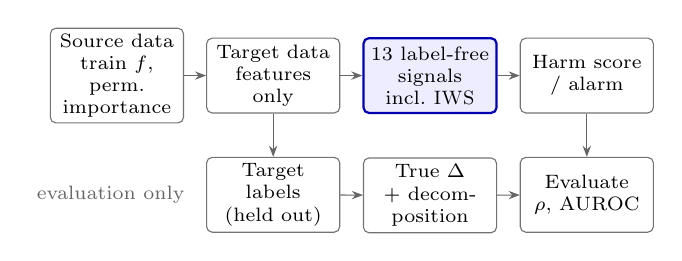
\begin{tikzpicture}[
  box/.style={draw=black!55, rounded corners=2pt, align=center, font=\scriptsize,
              minimum height=0.95cm, text width=1.55cm, inner sep=2pt},
  hl/.style={box, draw=blue!70!black, fill=blue!7, thick},
  arr/.style={-{Stealth[length=4pt]}, black!60}]
\node[box] (src) {Source data\\ train $f$, perm.\ importance};
\node[box, right=0.28cm of src] (tgt) {Target data\\ features only};
\node[hl, right=0.28cm of tgt] (sig) {13 label-free signals incl.\ \iws{}};
\node[box, right=0.28cm of sig] (harm) {Harm score / alarm};
\node[box, below=0.55cm of tgt] (lab) {Target labels\\ (held out)};
\node[box, below=0.55cm of sig] (dec) {True $\Delta$ + decomposition};
\node[box, below=0.55cm of harm] (ev) {Evaluate\\ $\rho$, AUROC};
\draw[arr] (src) -- (tgt); \draw[arr] (tgt) -- (sig); \draw[arr] (sig) -- (harm);
\draw[arr] (tgt) -- (lab); \draw[arr] (lab) -- (dec); \draw[arr] (dec) -- (ev); \draw[arr] (harm) -- (ev);
\node[font=\scriptsize, text=black!60, anchor=east] at ([xshift=-0.15cm]lab.west) {evaluation only};
\end{tikzpicture}
\caption{Study pipeline. The top row is what a deployed monitor sees; the bottom row exists only to score how well each signal predicts the real drop.}
\label{fig:pipeline}
\end{figure}

\subsection{Label-free signals}
We group thirteen signals by what they look at.

\textit{Data-only (D).} Mean and maximum per-feature KS statistic; mean per-feature Wasserstein-1 distance on source-standardized features; mean PSI with ten source-quantile bins; unbiased MMD$^2$ with an RBF kernel and median-heuristic bandwidth~\cite{gretton2012kernel}; and the AUC of a domain classifier (gradient-boosted trees, 3-fold cross-fitting) that separates source from target rows~\cite{lopezpaz2017c2st,rabanser2019failing}.

\textit{Model-aware drift (M), proposed.} Let $d_j$ be the drift of feature $j$ (KS statistic or standardized Wasserstein distance) and $I_j$ the permutation importance~\cite{fisher2019all,breiman2001random} of feature $j$ for model $f$, measured as the accuracy loss on source validation data when feature $j$ is shuffled. With $w_j=\max(I_j,0)/\sum_k \max(I_k,0)$,
\begin{equation}
\iws(f) \;=\; \sum_{j=1}^{p} w_j\, d_j .
\label{eq:iws}
\end{equation}
\iws{} is zero when only ignored features move and large when the features the model relies on move. It needs source labels once (for $w$) and no target labels. We report \iws{}-KS and \iws{}-Wass. The following observation motivates the weighting.

\begin{proposition}
Let $U\subseteq\{1,\dots,p\}$ be the features $f$ depends on, so $f(x)=g(x_U)$, and suppose $P_T(Y|X)=P_S(Y|X)$ with $P(Y|X)$ depending on $x$ only through $x_U$. If the shift leaves the marginal of $X_U$ unchanged, $P_T(x_U)=P_S(x_U)$, then $\Delta=0$, however large the drift of the features outside $U$.
\end{proposition}
\begin{proof}
$\mathrm{Acc}_D(f)=\mathbb{E}_{x_U\sim P_D}\big[P(Y{=}g(x_U)\mid x_U)\big]$ for $D\in\{S,T\}$. The integrand is the same function under $S$ and $T$, and so is the distribution it is integrated against; hence $\mathrm{Acc}_S=\mathrm{Acc}_T$.
\end{proof}

Data-only detectors respond to the drift of all $p$ features and so cannot respect this invariance; \iws{} approximates it by down-weighting features with zero importance. The converse does not hold: drift in $X_U$ can lower, leave unchanged or even raise accuracy (Sec.~\ref{sec:synth}), and a change in $P(Y|X)$ is invisible to any function of $X$ alone.

\textit{Model-output (O).} Drop in mean maximum class probability, i.e.\ difference of confidences (DoC)~\cite{guillory2021doc}; absolute change in predicted positive rate; ATC drop~\cite{garg2022atc}, i.e.\ source accuracy minus ATC's target estimate; importance-weighted drop (IW-drop), i.e.\ source accuracy minus the density-ratio-weighted source accuracy~\cite{shimodaira2000improving,sugiyama2007covariate}; and the increase in disagreement between $f$ and a reference model of a different class~\cite{baek2022agreement}.

\subsection{Covariate/conditional decomposition}
\label{sec:decomp}
The domain classifier gives out-of-fold probabilities $\hat p(T|x)$ for source rows, from which we form density-ratio weights $\hat r(x)=\frac{\hat p(T|x)}{1-\hat p(T|x)}\cdot\frac{n_S}{n_T}$ (probabilities clipped to $[0.01,0.99]$, weights capped at 50). The weighted source accuracy
\begin{equation}
\widehat{\mathrm{Acc}}_{S\to T}=\frac{\sum_i \hat r(x_i)\,\mathbb{1}[f(x_i)=y_i]}{\sum_i \hat r(x_i)}
\end{equation}
estimates what the target accuracy would be if only $P(X)$ had changed. We split
\begin{equation}
\Delta=\underbrace{\mathrm{Acc}_S-\widehat{\mathrm{Acc}}_{S\to T}}_{\text{covariate part}}
+\underbrace{\widehat{\mathrm{Acc}}_{S\to T}-\mathrm{Acc}_T}_{\text{residual (conditional) part}} .
\label{eq:decomp}
\end{equation}
The covariate part is label-free (it equals IW-drop); the residual needs target labels and is used only for analysis. When source and target barely overlap, reweighting cannot represent target regions absent from the source, so the residual also absorbs out-of-support error, which DISDE~\cite{cai2023diagnosing} treats as a separate term. We therefore also report results on the subset with domain-classifier AUC $<0.95$.

\subsection{Harm score}
To test whether signals combine, we fit a gradient-boosted regressor that maps all thirteen signals to $\Delta$. It is evaluated \emph{leave-one-dataset-out}: the regressor never sees any pair from the dataset it is scored on.

\begin{algorithm}[t]
\caption{Computing \iws{} for a deployed model}
\label{alg:iws}
\begin{algorithmic}[1]
\Require model $f$, source validation $(X_S,y_S)$, target batch $X_T$
\State $a \gets \mathrm{Acc}(f, X_S, y_S)$
\For{$j=1,\dots,p$} \Comment{once per model}
  \State $I_j \gets a - \mathrm{Acc}(f, \mathrm{shuffle}_j(X_S), y_S)$
\EndFor
\State $w_j \gets \max(I_j,0)/\sum_k \max(I_k,0)$
\For{each new target batch $X_T$}
  \State $d_j \gets \mathrm{KS}(X_S[:,j], X_T[:,j])$ for all $j$
  \State \Return $\iws=\sum_j w_j d_j$
\EndFor
\end{algorithmic}
\end{algorithm}

% =====================================================================
\section{Experimental Setup}
% =====================================================================
\subsection{Datasets and natural shifts}
We use seven public tabular datasets with natural domain structure (Table~\ref{tab:data}). Each split attribute defines domains; every ordered pair of domains with at least 400 rows becomes a source$\to$target pair, except temporal splits, where only past$\to$future pairs are kept. The split attribute itself is removed from the features. Bank Marketing has the known leakage variable ``duration'' removed and its calendar month removed for the time split. This yields 173 pairs.

\begin{table}[t]
\centering
\caption{Datasets and natural shift axes.}
\label{tab:data}
\footnotesize
\setlength{\tabcolsep}{3pt}
\begin{tabular}{lrrlr}
\toprule
Dataset & Rows & Feat. & Shift axes (domains) & Pairs \\
\midrule
Adult~\cite{kohavi1996scaling} & 45{,}222 & 48 & sex, race, age, education, workclass & 34 \\
COMPAS~\cite{angwin2016machine} & 6{,}172 & 13 & race, sex, age group & 14 \\
Housing~\cite{pace1997sparse} & 20{,}428 & 15 & ocean proximity, north/south & 14 \\
Bank~\cite{moro2014data} & 41{,}188 & 62 & time (6 blocks, 2008--10) & 15 \\
Elec2~\cite{harries1999splice} & 45{,}312 & 6 & time (8 blocks) & 28 \\
Airlines~\cite{ikonomovska2011learning} & 381{,}161 & 5 & carrier (top 8) & 56 \\
Covertype~\cite{blackard1999comparative} & 581{,}012 & 54 & wilderness area (4) & 12 \\
\bottomrule
\end{tabular}
\end{table}

\subsection{Models and protocol}
We train logistic regression, a histogram gradient-boosted tree ensemble (GBDT, the strongest model family on tabular data~\cite{grinsztajn2022tree,ke2017lightgbm}) and a two-layer MLP (128--64 units) with scikit-learn~\cite{pedregosa2011scikit}. Per source domain, up to 5{,}000 rows are held out for validation and up to 20{,}000 used for training; up to 5{,}000 target rows are sampled. Every pair is run with three seeds that change the sampling and model initialization, giving $173\times3\times3 = 1{,}557$ evaluations.

\subsection{Synthetic suite}
To validate signals and the decomposition against known ground truth, we draw $X\sim\mathcal{N}(0,I_{10})$ and $P(Y{=}1|x)=\sigma\big(2[1.5x_1+2\sin(1.5x_2)+x_1x_3-0.3]\big)$, so only $x_1,x_2,x_3$ matter. Five shift families are applied at magnitudes $m\in\{0,0.25,0.5,1,1.5,2\}$: (a) mean shift $+m$ of the seven ignored features; (b) mean shift $+m$ of the three used features; (c) spread: $x_2,x_3$ scaled by $1{+}m$, forcing extrapolation; (d) concept shift, where the $x_1$ coefficient is reduced by $1.5m$ with $P(X)$ fixed; and (e) label shift, where $P(Y{=}1)$ is moved to $0.5{+}0.2m$ by class-conditional resampling.

\subsection{Metrics}
Spearman $\rho$ between signal and $\Delta$, pooled over all evaluations (95\% bootstrap CI, 1{,}000 resamples) and averaged within each dataset$\times$model$\times$seed group; AUROC and AUPRC for detecting harmful shifts; and the false-positive rate at 90\% recall of harmful shifts (FPR@90). Paired comparisons use Wilcoxon signed-rank tests over the 63 groups with Holm correction.

% =====================================================================
\section{Results}
% =====================================================================
\subsection{How common is harmful drift?}
Shift is the norm, not the exception. Across the 1{,}557 evaluations the mean accuracy drop is 10.9\pp; 71\% exceed $\tau=2$\pp, while 17\% show a \emph{gain} in accuracy. A domain classifier separates source from target with AUC $\ge0.75$ in 87\% of evaluations and $\ge0.95$ in 68\%. A detector thresholded at AUC $0.75$ therefore alarms almost always, yet 25\% of those alarms are benign (339 of 1{,}353). Among the 204 evaluations with little drift, 48\% are still harmful: silent failures that no data-only detector can see. The alarm raises the harm rate only from 48\% to 75\%.

\subsection{Which signals track degradation? (RQ1)}
Table~\ref{tab:corr} ranks all signals. The model-aware \iws{} variants lead: \iws{}-Wass has the highest pooled and within-group correlation ($\rho=0.42$ and $0.36$), and \iws{}-KS the best harm detection (AUROC 0.70, AUPRC 0.86). Weighting by importance roughly doubles the correlation of plain KS (0.22$\to$0.40) and raises that of mean Wasserstein from 0.31 to 0.42. Fig.~\ref{fig:scatter} shows why the domain classifier, despite a similar pooled $\rho$, is a poor alarm: most pairs pile up at AUC $\approx1$, where it cannot rank them. Within that saturated subset \iws{}-KS still ranks drops better ($\rho=0.30$ vs.\ 0.22), and on unsaturated pairs the gap widens (0.30 vs.\ 0.15).

\begin{table}[t]
\centering
\caption{Rank correlation of each label-free signal with the accuracy drop and detection of harmful shifts ($\Delta>2$\pp), 1{,}557 evaluations. D = data-only, M = model-aware, O = model-output; $^\dagger$ proposed. Best underlined.}
\label{tab:corr}
\footnotesize
\setlength{\tabcolsep}{3pt}
\begin{tabular}{lcccc}
\toprule
Signal & $\rho$ pooled [95\% CI] & $\bar\rho$ within & AUROC & AUPRC \\
\midrule
IWS-Wass.$^\dagger$ (M) & \underline{0.42} [0.37, 0.46] & \underline{0.36} & 0.69 & 0.84 \\
Domain-clf. AUC (D) & 0.40 [0.35, 0.44] & 0.29 & 0.66 & 0.81 \\
IWS-KS$^\dagger$ (M) & 0.40 [0.35, 0.44] & 0.34 & \underline{0.70} & \underline{0.86} \\
KS (max) (D) & 0.35 [0.30, 0.39] & 0.28 & 0.62 & 0.80 \\
MMD$^2$ (D) & 0.33 [0.28, 0.37] & 0.26 & 0.63 & 0.82 \\
Wasserstein (mean) (D) & 0.31 [0.26, 0.34] & 0.27 & 0.65 & 0.82 \\
Prediction shift (O) & 0.28 [0.23, 0.33] & 0.27 & 0.60 & 0.81 \\
Disagreement incr. (O) & 0.25 [0.20, 0.30] & 0.29 & 0.63 & 0.82 \\
PSI (mean) (D) & 0.23 [0.17, 0.27] & 0.22 & 0.65 & 0.80 \\
KS (mean) (D) & 0.22 [0.18, 0.26] & 0.30 & 0.64 & 0.81 \\
Importance-wtd. drop (O) & 0.12 [0.07, 0.17] & 0.18 & 0.62 & 0.79 \\
ATC drop (O) & 0.07 [0.02, 0.12] & 0.08 & 0.58 & 0.80 \\
Confidence drop (DoC) (O) & 0.07 [0.02, 0.12] & 0.07 & 0.60 & 0.82 \\
\bottomrule
\end{tabular}
\end{table}

\begin{figure*}[t]
\centering
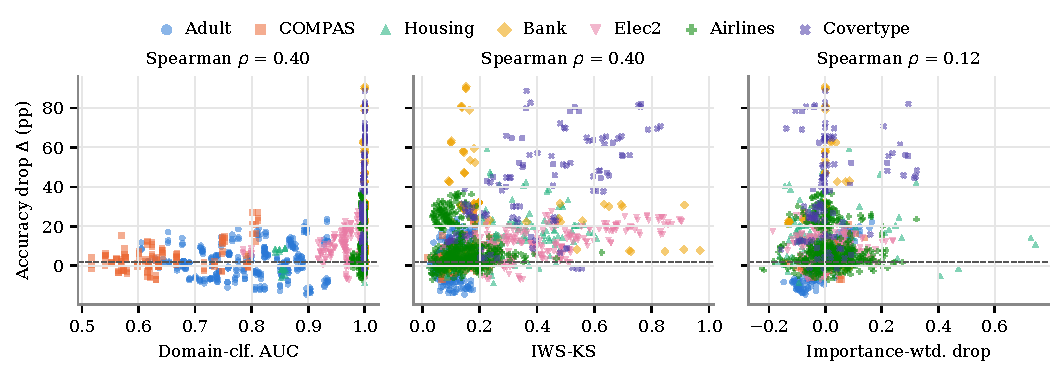
\includegraphics[width=\textwidth]{figures/fig_scatter.pdf}
\caption{Accuracy drop versus three signals for every evaluation. The domain-classifier AUC saturates at 1 for most natural shifts, so it cannot rank them; \iws{}-KS spreads the same pairs out. The density-ratio estimate (right) is close to zero for most harmful pairs because their loss comes from $P(Y|X)$. Dashed line: harm threshold $\tau=2$\pp.}
\label{fig:scatter}
\end{figure*}

Confidence-based estimators, which are among the best label-free accuracy predictors on image benchmarks~\cite{garg2022atc,guillory2021doc}, correlate weakly here: ATC drop $\rho=0.07$ and DoC $\rho=0.07$. Paired tests over the 63 groups confirm that \iws{}-KS beats PSI and MMD after Holm correction ($p_\text{Holm}<10^{-4}$ and $0.022$). Its advantages over mean KS (38 of 63 groups; pooled $\Delta\rho=+0.18$, 95\% CI $[0.13,0.23]$) and over ATC (pooled $\Delta\rho=+0.33$, CI $[0.26,0.39]$) have pooled bootstrap intervals that exclude zero but do not survive Holm correction at the group level ($p_\text{Holm}=0.11$ and $0.10$). Against the domain classifier, the pooled correlations are equal ($\Delta\rho=0.00$), and the AUROC/AUPRC advantage is not significant. We therefore claim that \iws{} is the most reliable single signal, not that it dominates every alternative.

\textit{No signal wins everywhere.} Table~\ref{tab:perds} breaks correlations down by dataset. Confidence-based signals are excellent on Adult (ATC $\rho=0.87$) and wrong-signed on Elec2 ($-0.50$), where the relation between demand and price direction drifts over time and the models stay confident while they fail. \iws{}-KS is best on Housing and Elec2 and positive on six of seven datasets; Airlines, where carrier changes alter delay patterns rather than inputs, defeats nearly all signals.

\begin{table}[t]
\centering
\caption{Within-dataset Spearman $\rho$ with $\Delta$ (all models and seeds).}
\label{tab:perds}
\footnotesize
\begin{tabular}{lccccc}
\toprule
Dataset & KS & DC-AUC & ATC & IW-drop & IWS-KS \\
\midrule
Adult & 0.02 & 0.05 & \underline{0.87} & 0.81 & 0.14 \\
COMPAS & 0.22 & \underline{0.32} & 0.28 & 0.27 & 0.26 \\
Housing & 0.44 & 0.38 & 0.26 & 0.04 & \underline{0.53} \\
Bank & \underline{0.45} & 0.31 & -0.12 & 0.01 & 0.44 \\
Elec2 & 0.46 & 0.15 & -0.50 & -0.01 & \underline{0.59} \\
Airlines & -0.22 & \underline{0.20} & -0.03 & -0.04 & -0.13 \\
Covertype & \underline{0.70} & 0.65 & 0.01 & 0.21 & 0.57 \\
\bottomrule
\end{tabular}
\end{table}

\subsection{Controlled shifts: when does drift hurt? (RQ2)}
\label{sec:synth}
Fig.~\ref{fig:synth} reports the synthetic suite (mean over three seeds and three models). (a) Shifting the seven ignored features drives the domain-classifier AUC to 1.0 while the drop stays at 1.0\pp; \iws{}-KS stays flat at 0.03, so it is the only drift signal that is not fooled. (b) Shifting the used features moves \iws{} strongly, yet accuracy \emph{improves} by 11.0\pp because the samples move away from the decision boundary. Drift in important features is therefore necessary for covariate-driven harm but not sufficient. (c) When the used features spread out and force extrapolation, the drop reaches 13.6\pp, and IW-drop (10.7\pp) and \iws{} both track it. (d) Under pure concept shift the drop reaches 28.8\pp while the domain-classifier AUC stays at 0.50: every label-free signal is blind, as theory predicts. (e) Label-prior shift changes $P(X)$ through $P(X|Y)$ but costs at most 1.5\pp.

\begin{figure*}[t]
\centering
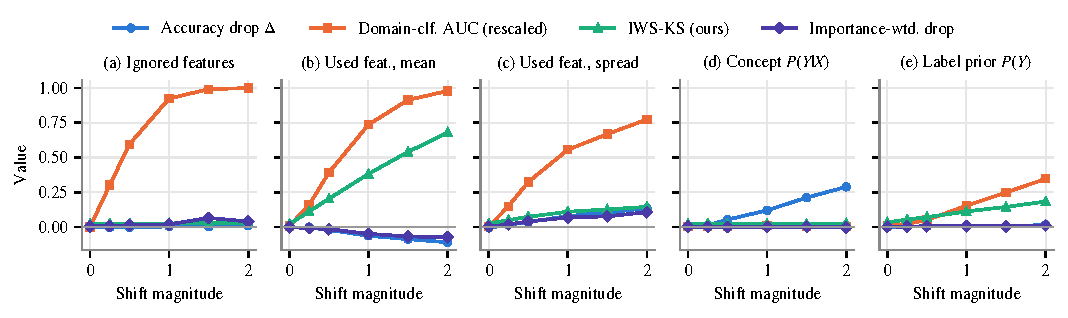
\includegraphics[width=\textwidth]{figures/fig_synthetic.pdf}
\caption{Synthetic shifts with known ground truth. Data-only drift (orange) reacts to every change in $P(X)$, harmful or not. \iws{} (green) ignores irrelevant drift (a) but cannot tell helpful from harmful movement of used features (b, c). No label-free signal sees concept shift (d).}
\label{fig:synth}
\end{figure*}

\subsection{Case study: the same drift statistic, opposite outcomes}
Fig.~\ref{fig:case} contrasts two natural pairs for GBDT. In Elec2 (time block 0$\to$7), the Victorian price, Victorian demand and inter-state transfer features drift heavily (KS 0.53--0.73), and the mean KS over all features is 0.36. The model, however, relies almost entirely on the New South Wales price ($w=0.95$, KS only 0.11), and accuracy is unchanged (81.7\%$\to$82.4\%). In Housing (coastal$\to$inland), mean KS is lower (0.20), but the drift falls on latitude, longitude and median income, the three features the model uses most, and accuracy collapses from 88.4\% to 61.3\%. Mean KS ranks the two pairs the wrong way round (0.36 vs.\ 0.20), whereas \iws{}-KS ranks them correctly (0.11 vs.\ 0.32).

\begin{figure*}[t]
\centering
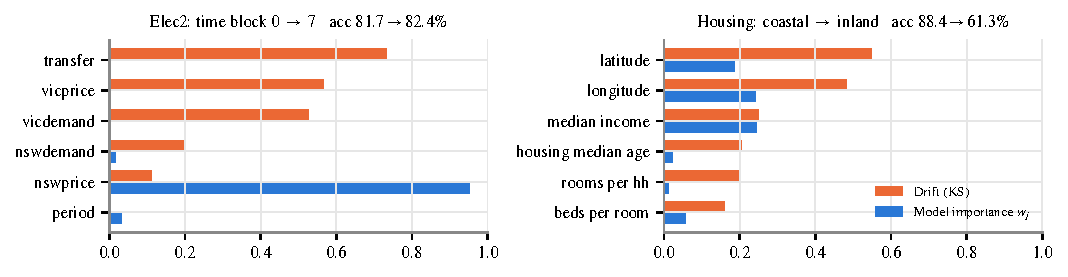
\includegraphics[width=0.92\textwidth]{figures/fig_case.pdf}
\caption{Per-feature drift (orange) and model importance (blue) for the six most-drifted features of two natural pairs (GBDT). Left: heavy drift in unused features, no harm. Right: moderate drift in the used features, a 27-point accuracy drop.}
\label{fig:case}
\end{figure*}

\subsection{What kind of shift causes the failures? (RQ3)}
The decomposition behaves correctly where the truth is known: under concept shift it assigns 29.2\pp of the 28.8\pp drop to the residual and $-0.3$\pp to the covariate part; under spread shift it assigns 10.7 of 13.6\pp to the covariate part. Its one failure mode is complete separation: with ignored features shifted by $m=2$ (AUC $=1.0$) it attributes a spurious 4.0\pp to covariate shift.

On the natural testbed (Fig.~\ref{fig:decomp}, Table~\ref{tab:decomp}) the residual part dominates the covariate part in 76\% of harmful evaluations and accounts for 55\% (Adult) to 94\% (Bank) of the mean absolute drop. Restricting to pairs with good overlap (AUC $<0.95$, 271 harmful evaluations) lowers but does not remove the dominance: 62\% of these are residual-dominated. This agrees with the finding of Liu~\textit{et~al.}~\cite{liu2023need} that $Y|X$ shifts dominate natural tabular shifts, and it explains the weak correlations above: the largest component of most drops is one that label-free signals cannot observe.

\begin{figure}[t]
\centering
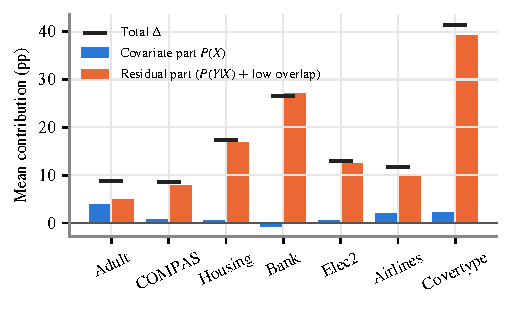
\includegraphics[width=\columnwidth]{figures/fig_decomposition.pdf}
\caption{Mean decomposition of harmful drops (Eq.~\ref{eq:decomp}). The residual, conditional part dominates on every dataset.}
\label{fig:decomp}
\end{figure}

\begin{table}[t]
\centering
\caption{Decomposition per dataset. Evals = pairs$\times$models$\times$seeds; $\bar\Delta_\text{harm}$ = mean drop of harmful evaluations (pp); $Y|X$ share = residual share of mean absolute drop; $|\pi_T-\pi_S|$ = mean change in positive rate.}
\label{tab:decomp}
\footnotesize
\setlength{\tabcolsep}{3.5pt}
\begin{tabular}{lrrrrr}
\toprule
Dataset & Evals & Harmful & $\bar\Delta_{\text{harm}}$ & $Y|X$ share & $|\pi_T-\pi_S|$ \\
\midrule
Adult & 306 & 49\% & 8.8 & 55\% & 0.134 \\
COMPAS & 126 & 56\% & 8.6 & 69\% & 0.141 \\
Housing & 126 & 81\% & 17.4 & 67\% & 0.246 \\
Bank & 135 & 79\% & 26.5 & 94\% & 0.125 \\
Elec2 & 252 & 86\% & 13.0 & 78\% & 0.043 \\
Airlines & 504 & 72\% & 11.7 & 70\% & 0.117 \\
Covertype & 108 & 97\% & 41.4 & 86\% & 0.267 \\
\bottomrule
\end{tabular}
\end{table}

\subsection{Can signals be combined into a harm score? (RQ4)}
Table~\ref{tab:harm} compares single signals with a meta-regressor evaluated leave-one-dataset-out. Learned combinations transfer poorly across datasets: data-only signals reach AUROC 0.55, adding \iws{} raises this to 0.59, and all thirteen signals reach 0.67 with $\rho=0.34$, still below \iws{}-KS alone (0.70, $\rho=0.40$). Fig.~\ref{fig:pr} shows \iws{}-KS holds precision above 0.9 up to about 30\% recall, the operating region relevant for a high-confidence ``retrain now'' alarm. At 90\% recall, however, every method raises false alarms on roughly three of four benign shifts (FPR@90 $\ge0.75$), a direct consequence of the conditional failures documented above.

\begin{table}[t]
\centering
\caption{Harm detection: single signals vs.\ a meta-regressor trained leave-one-dataset-out ($\Delta>2$\pp).}
\label{tab:harm}
\footnotesize
\setlength{\tabcolsep}{4pt}
\begin{tabular}{lcccc}
\toprule
Method & $\rho$ & AUROC & AUPRC & FPR@90 \\
\midrule
Domain-clf. AUC & 0.40 & 0.66 & 0.81 & 0.75 \\
ATC drop & 0.07 & 0.58 & 0.80 & 0.95 \\
Importance-wtd. drop & 0.12 & 0.62 & 0.79 & 0.83 \\
IWS-KS$^\dagger$ & 0.40 & 0.70 & 0.86 & 0.76 \\
\midrule \multicolumn{5}{l}{\emph{Meta-regressor, leave-one-dataset-out}} \\
Data-only signals & 0.13 & 0.55 & 0.75 & 0.84 \\
Data-only + IWS & 0.22 & 0.59 & 0.78 & 0.86 \\
All signals (harm score)$^\dagger$ & 0.34 & 0.67 & 0.83 & 0.81 \\
\bottomrule
\end{tabular}
\end{table}

\begin{figure}[t]
\centering
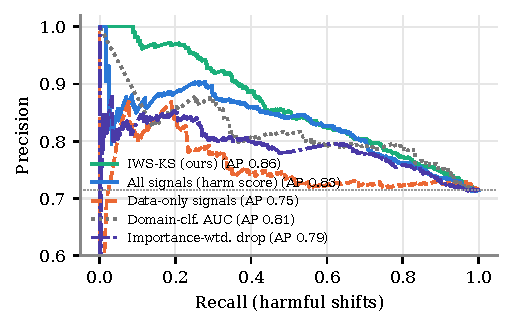
\includegraphics[width=\columnwidth]{figures/fig_pr.pdf}
\caption{Precision--recall for detecting harmful shifts. Dotted line: base rate (0.71).}
\label{fig:pr}
\end{figure}

\subsection{Ablations}
\label{sec:ablation}
\textit{Model class.} \iws{}-KS correlates with the drop for every model (GBDT 0.45, MLP 0.42, logistic regression 0.33), whereas ATC works only for GBDT (0.16) and is near zero for the other two (0.02), whose confidence is not informative of their errors under shift.
\textit{Harm threshold.} Varying $\tau\in\{1,2,5,10\}$\pp leaves the AUROC of \iws{}-KS between 0.70 and 0.71, while ATC falls from 0.60 to 0.49 and the domain classifier stays at 0.66--0.69. \iws{} is thus robust to how ``harmful'' is defined.
\textit{Target sample size.} Monitoring often has to act on small batches. Table~\ref{tab:nsize} recomputes four signals for GBDT (seed 0, all 173 pairs) on $n_T\in\{100,300,1000,5000\}$ unlabelled target rows, always scoring against the drop measured on the full sample. \iws{}-KS keeps the highest rank correlation at every size ($\rho=0.45$--$0.47$), and its AUROC with only 100 rows (0.73) matches that with 5{,}000 rows. Mean KS is similarly stable and, in this GBDT-only setting, reaches comparable AUROC (0.72--0.74) at a lower correlation. ATC degrades most at small $n_T$ ($\rho=0.06$ at 100 rows).

\begin{table}[t]
\centering
\caption{Effect of the number of unlabelled target rows $n_T$ (GBDT, seed 0, 173 pairs). Cells: Spearman $\rho$ / AUROC for harm ($\Delta>2$\pp).}
\label{tab:nsize}
\footnotesize
\setlength{\tabcolsep}{3.5pt}
\begin{tabular}{rcccc}
\toprule
$n_T$ & KS (mean) & DC-AUC & ATC drop & IWS-KS$^\dagger$ \\
\midrule
100 & 0.28 / 0.72 & 0.42 / 0.68 & 0.06 / 0.59 & 0.47 / 0.73 \\
300 & 0.30 / 0.74 & 0.43 / 0.69 & 0.13 / 0.64 & 0.46 / 0.72 \\
1{,}000 & 0.30 / 0.73 & 0.43 / 0.69 & 0.16 / 0.64 & 0.46 / 0.72 \\
5{,}000 & 0.30 / 0.73 & 0.43 / 0.70 & 0.15 / 0.64 & 0.45 / 0.72 \\
\bottomrule
\end{tabular}
\end{table}

% =====================================================================
\section{Discussion}
% =====================================================================
\textit{A taxonomy of failure.} Combining drift magnitude (domain-classifier AUC $\ge0.75$), harm ($\Delta>2$\pp) and the dominant decomposition term places each evaluation in one of four regimes: \emph{stable} (7\%), \emph{benign drift} (22\%), \emph{harmful covariate shift} (17\%) and \emph{conditional failure} (54\%). Only the third is what drift detectors are designed for; the second wastes retraining effort and the fourth goes unnoticed. Table~\ref{tab:tax} shows the mix differs sharply by shift axis. Demographic splits (Adult, COMPAS) contain the most stable and benign cases, whereas temporal and geographic splits (Bank, Elec2, Covertype) are dominated by conditional failures, the regime in which unlabelled monitoring is weakest.

\begin{table}[t]
\centering
\caption{Failure regimes per dataset (share of evaluations). High drift = domain-classifier AUC $\ge0.75$; harmful = $\Delta>2$\pp; covariate vs.\ conditional by the larger term of Eq.~\eqref{eq:decomp}.}
\label{tab:tax}
\footnotesize
\setlength{\tabcolsep}{3.5pt}
\begin{tabular}{lrrrr}
\toprule
Dataset & Stable & Benign drift & Harmful cov. & Conditional \\
\midrule
Adult & 19\% & 33\% & 21\% & 28\% \\
COMPAS & 39\% & 6\% & 10\% & 45\% \\
Housing & 0\% & 19\% & 17\% & 63\% \\
Bank & 0\% & 21\% & 2\% & 77\% \\
Elec2 & 0\% & 14\% & 14\% & 72\% \\
Airlines & 0\% & 28\% & 24\% & 48\% \\
Covertype & 0\% & 3\% & 10\% & 87\% \\
\midrule All & 7\% & 22\% & 17\% & 54\% \\
\bottomrule
\end{tabular}
\end{table}

\textit{Practical guidance.} (i) Replace raw per-feature drift dashboards with importance-weighted drift: it costs one permutation-importance pass per model and filters out drift in ignored features. (ii) Do not rely on model confidence for tabular monitoring; ATC and DoC were wrong-signed on temporal data. (iii) Because conditional shift dominates, budget for a small stream of delayed labels; no amount of unlabelled monitoring recovers a change in $P(Y|X)$. (iv) Treat a saturated domain classifier as ``the data changed'', never as ``the model broke''.

\textit{Limitations and threats to validity.} Our testbed covers seven datasets and binary classification; regression and high-dimensional data may behave differently. Pairs from the same dataset are not independent, which is why we report within-group statistics and leave-one-dataset-out results. The decomposition relies on density-ratio estimation and is unreliable under near-complete separation, as our synthetic check shows. Permutation importance is computed on source data; under strong shift the features the model relies on may change, and conditional importance~\cite{lundberg2017unified} could refine Eq.~\eqref{eq:iws}. Finally, the strongest recent estimators (PAPE~\cite{bialek2025pape}, Detectron~\cite{ginsberg2023detectron}) were not re-implemented; IW-drop and disagreement serve as their simpler counterparts.

% =====================================================================
\section{Conclusion}
% =====================================================================
Feature-space change predicts model failure only weakly on natural tabular shifts. Drift is nearly universal, a quarter of drift alarms are benign, and most harmful drops come from a change in $P(Y|X)$ that unlabelled data cannot reveal. Weighting drift by what the model actually uses (\iws{}) is the most reliable label-free signal we tested and is trivial to deploy, but the dominant failure mode calls for monitoring that combines model-aware drift with a small budget of fresh labels. Code, raw results and scripts that regenerate every table and figure are released with the paper.

\balance
% Bibliography embedded so this file compiles without refs.bib
% Generated by IEEEtran.bst, version: 1.14 (2015/08/26)
\begin{thebibliography}{10}
\providecommand{\url}[1]{#1}
\csname url@samestyle\endcsname
\providecommand{\newblock}{\relax}
\providecommand{\bibinfo}[2]{#2}
\providecommand{\BIBentrySTDinterwordspacing}{\spaceskip=0pt\relax}
\providecommand{\BIBentryALTinterwordstretchfactor}{4}
\providecommand{\BIBentryALTinterwordspacing}{\spaceskip=\fontdimen2\font plus
\BIBentryALTinterwordstretchfactor\fontdimen3\font minus
  \fontdimen4\font\relax}
\providecommand{\BIBforeignlanguage}[2]{{%
\expandafter\ifx\csname l@#1\endcsname\relax
\typeout{** WARNING: IEEEtran.bst: No hyphenation pattern has been}%
\typeout{** loaded for the language `#1'. Using the pattern for}%
\typeout{** the default language instead.}%
\else
\language=\csname l@#1\endcsname
\fi
#2}}
\providecommand{\BIBdecl}{\relax}
\BIBdecl

\bibitem{quinonero2009dataset}
J.~Qui{\~n}onero-Candela, M.~Sugiyama, A.~Schwaighofer, and N.~D. Lawrence,
  Eds., \emph{Dataset Shift in Machine Learning}.\hskip 1em plus 0.5em minus
  0.4em\relax MIT Press, 2009.

\bibitem{moreno2012unifying}
J.~G. Moreno-Torres, T.~Raeder, R.~Alaiz-Rodr{\'\i}guez, N.~V. Chawla, and
  F.~Herrera, ``A unifying view on dataset shift in classification,''
  \emph{Pattern Recognition}, vol.~45, no.~1, pp. 521--530, 2012.

\bibitem{gretton2012kernel}
A.~Gretton, K.~M. Borgwardt, M.~J. Rasch, B.~Sch{\"o}lkopf, and A.~Smola, ``A
  kernel two-sample test,'' \emph{Journal of Machine Learning Research},
  vol.~13, pp. 723--773, 2012.

\bibitem{lopezpaz2017c2st}
D.~Lopez-Paz and M.~Oquab, ``Revisiting classifier two-sample tests,'' in
  \emph{International Conference on Learning Representations (ICLR)}, 2017.

\bibitem{rabanser2019failing}
S.~Rabanser, S.~G{\"u}nnemann, and Z.~C. Lipton, ``Failing loudly: An empirical
  study of methods for detecting dataset shift,'' in \emph{Advances in Neural
  Information Processing Systems (NeurIPS)}, vol.~32, 2019.

\bibitem{liu2023need}
J.~Liu, T.~Wang, P.~Cui, and H.~Namkoong, ``On the need for a language
  describing distribution shifts: Illustrations on tabular datasets,'' in
  \emph{Advances in Neural Information Processing Systems (NeurIPS), Datasets
  and Benchmarks Track}, 2023.

\bibitem{gardner2023tableshift}
J.~Gardner, Z.~Popovic, and L.~Schmidt, ``Benchmarking distribution shift in
  tabular data with {TableShift},'' in \emph{Advances in Neural Information
  Processing Systems (NeurIPS), Datasets and Benchmarks Track}, 2023.

\bibitem{gama2004ddm}
J.~Gama, P.~Medas, G.~Castillo, and P.~Rodrigues, ``Learning with drift
  detection,'' in \emph{Advances in Artificial Intelligence -- SBIA 2004}, ser.
  Lecture Notes in Computer Science, vol. 3171.\hskip 1em plus 0.5em minus
  0.4em\relax Springer, 2004, pp. 286--295.

\bibitem{gama2014survey}
J.~Gama, I.~{\v{Z}}liobait{\.e}, A.~Bifet, M.~Pechenizkiy, and A.~Bouchachia,
  ``A survey on concept drift adaptation,'' \emph{ACM Computing Surveys},
  vol.~46, no.~4, pp. 44:1--44:37, 2014.

\bibitem{lu2019learning}
J.~Lu, A.~Liu, F.~Dong, F.~Gu, J.~Gama, and G.~Zhang, ``Learning under concept
  drift: A review,'' \emph{IEEE Transactions on Knowledge and Data
  Engineering}, vol.~31, no.~12, pp. 2346--2363, 2019.

\bibitem{webb2016characterizing}
G.~I. Webb, R.~Hyde, H.~Cao, H.~L. Nguyen, and F.~Petitjean, ``Characterizing
  concept drift,'' \emph{Data Mining and Knowledge Discovery}, vol.~30, no.~4,
  pp. 964--994, 2016.

\bibitem{garg2022atc}
S.~Garg, S.~Balakrishnan, Z.~C. Lipton, B.~Neyshabur, and H.~Sedghi,
  ``Leveraging unlabeled data to predict out-of-distribution performance,'' in
  \emph{International Conference on Learning Representations (ICLR)}, 2022.

\bibitem{guillory2021doc}
D.~Guillory, V.~Shankar, S.~Ebrahimi, T.~Darrell, and L.~Schmidt, ``Predicting
  with confidence on unseen distributions,'' in \emph{Proceedings of the
  IEEE/CVF International Conference on Computer Vision (ICCV)}, 2021, pp.
  1134--1144.

\bibitem{baek2022agreement}
C.~Baek, Y.~Jiang, A.~Raghunathan, and J.~Z. Kolter, ``Agreement-on-the-line:
  Predicting the performance of neural networks under distribution shift,'' in
  \emph{Advances in Neural Information Processing Systems (NeurIPS)}, vol.~35,
  2022.

\bibitem{miller2021accuracy}
J.~Miller, R.~Taori, A.~Raghunathan, S.~Sagawa, P.~W. Koh, V.~Shankar,
  P.~Liang, Y.~Carmon, and L.~Schmidt, ``Accuracy on the line: On the strong
  correlation between out-of-distribution and in-distribution generalization,''
  in \emph{Proceedings of the 38th International Conference on Machine Learning
  (ICML)}, ser. PMLR, vol. 139, 2021.

\bibitem{shimodaira2000improving}
H.~Shimodaira, ``Improving predictive inference under covariate shift by
  weighting the log-likelihood function,'' \emph{Journal of Statistical
  Planning and Inference}, vol.~90, no.~2, pp. 227--244, 2000.

\bibitem{sugiyama2007covariate}
M.~Sugiyama, M.~Krauledat, and K.-R. M{\"u}ller, ``Covariate shift adaptation
  by importance weighted cross validation,'' \emph{Journal of Machine Learning
  Research}, vol.~8, pp. 985--1005, 2007.

\bibitem{bialek2025pape}
J.~Bia{\l}ek, J.~Kivim{\"a}ki, W.~Kuberski, and N.~Perrakis, ``Estimating model
  performance under covariate shift without labels,'' in \emph{Advances in
  Neural Information Processing Systems (NeurIPS)}, 2025.

\bibitem{koh2021wilds}
P.~W. Koh \emph{et~al.}, ``{WILDS}: A benchmark of in-the-wild distribution
  shifts,'' in \emph{Proceedings of the 38th International Conference on
  Machine Learning (ICML)}, ser. PMLR, vol. 139, 2021.

\bibitem{podkopaev2022tracking}
A.~Podkopaev and A.~Ramdas, ``Tracking the risk of a deployed model and
  detecting harmful distribution shifts,'' in \emph{International Conference on
  Learning Representations (ICLR)}, 2022.

\bibitem{ginsberg2023detectron}
T.~Ginsberg, Z.~Liang, and R.~G. Krishnan, ``A learning based hypothesis test
  for harmful covariate shift,'' in \emph{International Conference on Learning
  Representations (ICLR)}, 2023.

\bibitem{amoukou2024sequential}
S.~I. Amoukou, T.~Bewley, S.~Mishra, F.~Lecue, D.~Magazzeni, and M.~Veloso,
  ``Sequential harmful shift detection without labels,'' in \emph{Advances in
  Neural Information Processing Systems (NeurIPS)}, 2024.

\bibitem{zhang2023why}
H.~Zhang, H.~Singh, M.~Ghassemi, and S.~Joshi, ````{W}hy did the model fail?'':
  Attributing model performance changes to distribution shifts,'' in
  \emph{Proceedings of the 40th International Conference on Machine Learning
  (ICML)}, ser. PMLR, vol. 202, 2023.

\bibitem{cai2023diagnosing}
T.~T. Cai, H.~Namkoong, and S.~Yadlowsky, ``Diagnosing model performance under
  distribution shift,'' arXiv:2303.02011, 2023.

\bibitem{kulinski2023explaining}
S.~Kulinski and D.~I. Inouye, ``Towards explaining distribution shifts,'' in
  \emph{Proceedings of the 40th International Conference on Machine Learning
  (ICML)}, ser. PMLR, vol. 202, 2023.

\bibitem{mougan2022explanation}
C.~Mougan, K.~Broelemann, G.~Kasneci, T.~Tiropanis, and S.~Staab, ``Explanation
  shift: Detecting distribution shifts on tabular data via the explanation
  space,'' in \emph{NeurIPS Workshop on Distribution Shifts: Connecting Methods
  and Applications}, 2022.

\bibitem{lundberg2017unified}
S.~M. Lundberg and S.-I. Lee, ``A unified approach to interpreting model
  predictions,'' in \emph{Advances in Neural Information Processing Systems
  (NeurIPS)}, vol.~30, 2017.

\bibitem{zafar2026fmmo}
M.~R. Zafar, A.~El-Sharif, and N.~Khan, ``{FMMO}: Detecting the divergence
  between local attribution and global drift,'' arXiv:2609.06173, 2026.

\bibitem{lipton2018bbse}
Z.~C. Lipton, Y.-X. Wang, and A.~J. Smola, ``Detecting and correcting for label
  shift with black box predictors,'' in \emph{Proceedings of the 35th
  International Conference on Machine Learning (ICML)}, ser. PMLR, vol.~80,
  2018.

\bibitem{fisher2019all}
A.~Fisher, C.~Rudin, and F.~Dominici, ``All models are wrong, but many are
  useful: Learning a variable's importance by studying an entire class of
  prediction models simultaneously,'' \emph{Journal of Machine Learning
  Research}, vol.~20, no. 177, pp. 1--81, 2019.

\bibitem{breiman2001random}
L.~Breiman, ``Random forests,'' \emph{Machine Learning}, vol.~45, no.~1, pp.
  5--32, 2001.

\bibitem{kohavi1996scaling}
R.~Kohavi, ``Scaling up the accuracy of naive-{B}ayes classifiers: A
  decision-tree hybrid,'' in \emph{Proceedings of the 2nd International
  Conference on Knowledge Discovery and Data Mining (KDD)}, 1996, pp. 202--207.

\bibitem{angwin2016machine}
J.~Angwin, J.~Larson, S.~Mattu, and L.~Kirchner, ``Machine bias,'' ProPublica,
  2016.

\bibitem{pace1997sparse}
R.~K. Pace and R.~Barry, ``Sparse spatial autoregressions,'' \emph{Statistics
  \& Probability Letters}, vol.~33, no.~3, pp. 291--297, 1997.

\bibitem{moro2014data}
S.~Moro, P.~Cortez, and P.~Rita, ``A data-driven approach to predict the
  success of bank telemarketing,'' \emph{Decision Support Systems}, vol.~62,
  pp. 22--31, 2014.

\bibitem{harries1999splice}
M.~Harries, ``{SPLICE-2} comparative evaluation: Electricity pricing,'' The
  University of New South Wales, Tech. Rep., 1999.

\bibitem{ikonomovska2011learning}
E.~Ikonomovska, J.~Gama, and S.~D{\v{z}}eroski, ``Learning model trees from
  evolving data streams,'' \emph{Data Mining and Knowledge Discovery}, vol.~23,
  no.~1, pp. 128--168, 2011.

\bibitem{blackard1999comparative}
J.~A. Blackard and D.~J. Dean, ``Comparative accuracies of artificial neural
  networks and discriminant analysis in predicting forest cover types from
  cartographic variables,'' \emph{Computers and Electronics in Agriculture},
  vol.~24, no.~3, pp. 131--151, 1999.

\bibitem{grinsztajn2022tree}
L.~Grinsztajn, E.~Oyallon, and G.~Varoquaux, ``Why do tree-based models still
  outperform deep learning on typical tabular data?'' in \emph{Advances in
  Neural Information Processing Systems (NeurIPS), Datasets and Benchmarks
  Track}, 2022.

\bibitem{ke2017lightgbm}
G.~Ke, Q.~Meng, T.~Finley, T.~Wang, W.~Chen, W.~Ma, Q.~Ye, and T.-Y. Liu,
  ``{LightGBM}: A highly efficient gradient boosting decision tree,'' in
  \emph{Advances in Neural Information Processing Systems (NeurIPS)}, vol.~30,
  2017.

\bibitem{pedregosa2011scikit}
F.~Pedregosa \emph{et~al.}, ``Scikit-learn: Machine learning in {P}ython,''
  \emph{Journal of Machine Learning Research}, vol.~12, pp. 2825--2830, 2011.

\end{thebibliography}

\end{document}
